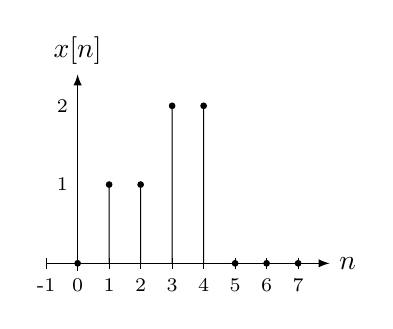
\begin{tikzpicture}
    \draw[-latex] (-1*0.4,0) -- (8*0.4,0) node[anchor=west] {$n$};
    \draw[-latex] (0, -0.1) -- ++(0,2.5) node[anchor=south] {$x[n]$};
    \foreach \x in {0}
        {
            \draw[fill=black] (\x*0.4, 0) circle (1pt);
        }
    \foreach \x in {1,2}
        {
            \draw[fill=black] (\x*0.4, 0)  -- ++(0,1) circle (1pt);
        }
    \foreach \x in {3,4}
        {
            \draw[fill=black] (\x*0.4, 0)  -- ++(0,2) circle (1pt);
        }        
        
    \foreach \x in {5,6,7}
        {
            \draw[fill=black] (\x*0.4, 0) circle (1pt);
        }        
    \foreach \x in {-1, 0, ..., 7}
    {
        \draw (\x*0.4, 2pt) -- ++(0, -4pt) node[anchor=north]{\scriptsize \x};
    }
    \foreach \y in {1,2}
    {    
    	\node at (0,\y) [anchor=east] {\scriptsize \y};
    }
\end{tikzpicture}